\title{CSCI-580 Assignment 1}
\author{Ian Stewart}
\date{September 12, 2024}
\documentclass{article}

% Adjusts paper size
\usepackage[a4paper, total={6.2in, 8in}]{geometry}

% Packages + setup for graphs & captions
\usepackage{tikz}
\usepackage{caption}
\captionsetup[table]{skip=0pt,singlelinecheck=off}
\usetikzlibrary{arrows.meta}

\begin{document}
\maketitle

\section*{Part 1}
Use the A* algorithm to find a path between nodes S and G.
\begin{center}
    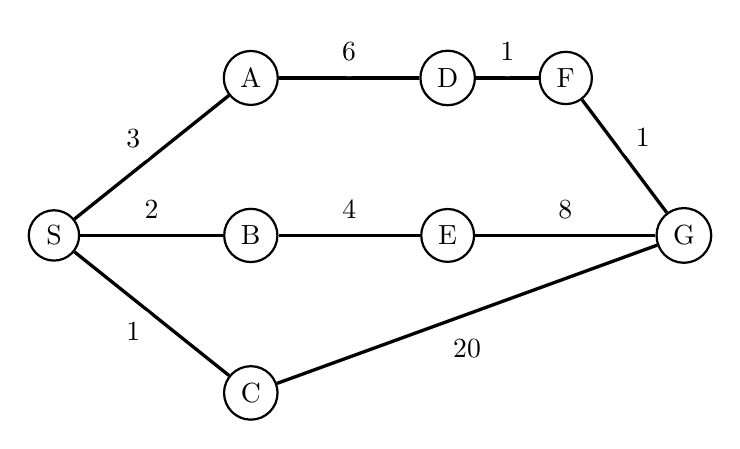
\begin{tikzpicture}
        \begin{scope}[every node/.style={circle,thick,draw}]
            \node (S) at (0,0) {S};
            \node (A) at (2.5,2) {A};
            \node (B) at (2.5,0) {B};
            \node (C) at (2.5,-2) {C};
            \node (D) at (5,2) {D};
            \node (E) at (5,0) {E};
            \node (F) at (6.5,2) {F};
            \node (G) at (8,0) {G};
        \end{scope}
        
        \begin{scope}[>={Stealth[black]},
                    every node/.style={fill=white,circle},
                    every edge/.style={draw=black,very thick}]
            \path [-] (S) edge node [above left] {$3$} (A);
            \path [-] (S) edge node [above]      {$2$} (B);
            \path [-] (S) edge node [below left] {$1$} (C);
            \path [-] (A) edge node [above]      {$6$} (D);
            \path [-] (B) edge node [above]      {$4$} (E);
            \path [-] (C) edge node [below, yshift=-1]{$20$} (G);
            \path [-] (D) edge node [above]      {$1$} (F);
            \path [-] (F) edge node [above right]{$1$} (G);
            \path [-] (E) edge node [above]      {$8$} (G);
        \end{scope}
    \end{tikzpicture}
\end{center}

\begin{table}
    \caption*{Heuristic:}
    \begin{tabular}{|c|c|}
        \hline\hline
        $n$ & $h(n)$ \\
        \hline\hline
        A & 7  \\
        \hline
        B & 10 \\
        \hline
        C & 15 \\
        \hline
        D & 1  \\
        \hline
        E & 8  \\
        \hline
        F & 1  \\
        \hline
        G & 0  \\
        \hline
        S & 10 \\
        \hline
    \end{tabular}
\end{table}

\pagebreak
\subsection*{Steps:}

\begin{table}[!h]
    \caption*{Path Evaluation}
    \begin{tabular}{|c|c|c|c|c|}
        \hline\hline
        Path & $g(n) +$ & $h(n)$ & $\Rightarrow f(n)$ & Shortest \\
        \hline\hline
        $S \rightarrow A$ & 3 & 7 & 10 & 10\\
        \hline
        $S \rightarrow B$ & 2 & 10 & 12 & \\
        \hline
        $S \rightarrow C$ & 1 & 15 & 16 & \\
        \hline
        $S \rightarrow A \rightarrow D$ & 9 & 1 & 10 & 10\\
        \hline
        $S \rightarrow A \rightarrow D \rightarrow F$ & 10 & 1 & 11 & 11\\
        \hline
        $S \rightarrow A \rightarrow D \rightarrow F \rightarrow G$ & 11 & 0 & 11 & 11\\
        \hline
    \end{tabular}
\end{table}

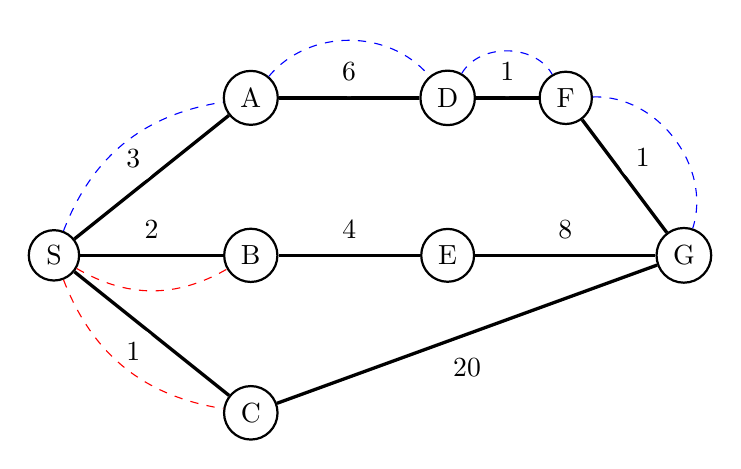
\begin{tikzpicture}
    \begin{scope}[every node/.style={circle,thick,draw}]
        \node (S) at (0,0) {S};
        \node (A) at (2.5,2) {A};
        \node (B) at (2.5,0) {B};
        \node (C) at (2.5,-2) {C};
        \node (D) at (5,2) {D};
        \node (E) at (5,0) {E};
        \node (F) at (6.5,2) {F};
        \node (G) at (8,0) {G};
    \end{scope}
    
    \begin{scope}[>={Stealth[black]},
                  every node/.style={fill=white,circle},
                  every edge/.style={draw=black,very thick}]
        \path [-] (S) edge node [above left] {$3$} (A);
        \path [-] (S) edge node [above]      {$2$} (B);
        \path [-] (S) edge node [below left] {$1$} (C);
        \path [-] (A) edge node [above]      {$6$} (D);
        \path [-] (B) edge node [above]      {$4$} (E);
        \path [-] (C) edge node [below, yshift=-1]{$20$} (G);
        \path [-] (D) edge node [above]      {$1$} (F);
        \path [-] (F) edge node [above right]{$1$} (G);
        \path [-] (E) edge node [above]      {$8$} (G);
    \end{scope}

    % Blue dashed edges showing the path found by A*
    \begin{scope}[>={Stealth[black]},
            every edge/.style={draw=blue, dashed}]
        \path [bend left] (S) edge (A);
        \path [bend left=50] (A) edge (D);
        \path [bend left=60] (D) edge (F);
        \path [bend left=55] (F) edge (G);
    \end{scope}

    % Red dashed edges showing abandoned paths
    \begin{scope}[>={Stealth[black]},
        every edge/.style={draw=red, dashed}]
        \path [bend right] (S) edge (B);
        \path [bend right] (S) edge (C);
    \end{scope}
\end{tikzpicture}

\vspace*{1em}
\noindent The resulting path, as shown above in blue, is $S \rightarrow A \rightarrow D \rightarrow F \rightarrow G$.
The red paths are those that were not explored further because the cost $f(n)$ was too large.

\section*{Part 2}
\begin{enumerate}
    \item \textbf{Is h admissible?} \\
    Yes, h is admissible because the true cost from any node to the 
    goal node is never overestimated by the heuristic.
    \item \textbf{Is h consistent?} \\
    Yes, h is consistent because for each node the inequality
    $h(n) \leq c(n, n') + h(n')$ is satisfied. \\
    Using $S \rightarrow A$ as an example, $h(S) = 10$, $c(S, A) = 3$,
    and $h(A) = 7$. Since $10 \leq 3 + 7$, consistency holds for this 
    node. This is true for all nodes in this graph.
    \item \textbf{Is A* optimal for this problem?} \\
    Yes, A* is optimal for this problem because the heuristic used is 
    both admissible and consistent.
\end{enumerate}

\end{document}
